% This must be in the first 5 lines to tell arXiv to use pdfLaTeX, which is strongly recommended.
\pdfoutput=1
% In particular, the hyperref package requires pdfLaTeX in order to break URLs across lines.

\documentclass[11pt]{article}

% Change "review" to "final" to generate the final (sometimes called camera-ready) version.
% Change to "preprint" to generate a non-anonymous version with page numbers.
\usepackage[preprint]{acl}

% Standard package includes
\usepackage{times}
\usepackage{latexsym}

% For proper rendering and hyphenation of words containing Latin characters (including in bib files)
\usepackage[T1]{fontenc}
% For Vietnamese characters
% \usepackage[T5]{fontenc}
% See https://www.latex-project.org/help/documentation/encguide.pdf for other character sets

% This assumes your files are encoded as UTF8
\usepackage[utf8]{inputenc}

% This is not strictly necessary, and may be commented out,
% but it will improve the layout of the manuscript,
% and will typically save some space.
\usepackage{microtype}

% This is also not strictly necessary, and may be commented out.
% However, it will improve the aesthetics of text in
% the typewriter font.
\usepackage{inconsolata}

%Including images in your LaTeX document requires adding
%additional package(s)
\usepackage{graphicx}

% If the title and author information does not fit in the area allocated, uncomment the following
%
%\setlength\titlebox{<dim>}
%
% and set <dim> to something 5cm or larger.

\title{"All the world's a stage, and all the agents merely players": Persona Driven Survey Response Generation}

% Author information can be set in various styles:
% For several authors from the same institution:
\author{Arya Shah, Swaraj Bhanja, Suryansh Srivastava \\
         Department of Computer Science and Information Management\\ Asian Institute of Technology \\ Pathumthani, Thailand \\ \texttt{{{st125462, st125052, st14997}@ait.ac.th}}}
% if the names do not fit well on one line use
%         Author 1 \\ {\bf Author 2} \\ ... \\ {\bf Author n} \\
% For authors from different institutions:
% \author{Author 1 \\ Address line \\  ... \\ Address line
%         \And  ... \And
%         Author n \\ Address line \\ ... \\ Address line}
% To start a separate ``row'' of authors use \AND, as in
% \author{Author 1 \\ Address line \\  ... \\ Address line
%         \AND
%         Author 2 \\ Address line \\ ... \\ Address line \And
%         Author 3 \\ Address line \\ ... \\ Address line}

%\author{Arya Shah \\
  %Department of Computer Science and Information Management \\
  %Asian Institute of Technology\\
  %Pathumthani, Thailand \\
  %\texttt{st125462@ait.ac.th} \\\And
  %Second Author \\
  %Affiliation / Address line 1 \\
  %Affiliation / Address line 2 \\
  %Affiliation / Address line 3 \\
  %\texttt{email@domain} \\}

%\author{
%  \textbf{First Author\textsuperscript{1}},
%  \textbf{Second Author\textsuperscript{1,2}},
%  \textbf{Third T. Author\textsuperscript{1}},
%  \textbf{Fourth Author\textsuperscript{1}},
%\\
%  \textbf{Fifth Author\textsuperscript{1,2}},
%  \textbf{Sixth Author\textsuperscript{1}},
%  \textbf{Seventh Author\textsuperscript{1}},
%  \textbf{Eighth Author \textsuperscript{1,2,3,4}},
%\\
%  \textbf{Ninth Author\textsuperscript{1}},
%  \textbf{Tenth Author\textsuperscript{1}},
%  \textbf{Eleventh E. Author\textsuperscript{1,2,3,4,5}},
%  \textbf{Twelfth Author\textsuperscript{1}},
%\\
%  \textbf{Thirteenth Author\textsuperscript{3}},
%  \textbf{Fourteenth F. Author\textsuperscript{2,4}},
%  \textbf{Fifteenth Author\textsuperscript{1}},
%  \textbf{Sixteenth Author\textsuperscript{1}},
%\\
%  \textbf{Seventeenth S. Author\textsuperscript{4,5}},
%  \textbf{Eighteenth Author\textsuperscript{3,4}},
%  \textbf{Nineteenth N. Author\textsuperscript{2,5}},
%  \textbf{Twentieth Author\textsuperscript{1}}
%\\
%\\
%  \textsuperscript{1}Affiliation 1,
%  \textsuperscript{2}Affiliation 2,
%  \textsuperscript{3}Affiliation 3,
%  \textsuperscript{4}Affiliation 4,
%  \textsuperscript{5}Affiliation 5
%\\
%  \small{
%    \textbf{Correspondence:} \href{mailto:email@domain}{email@domain}
%  }
%}

\begin{document}
\maketitle
\begin{abstract}
One of the crucial frameworks for understanding various human behavior, attitude, and opinion is the conduction of surveys, which can contain responses across a number of diverse disciplines such as human-computer interaction, social science, market research and psychological traits, to name a few. However, the collection of diverse survey responses on a large scale remains to be a challenge across many domains which include difficulties in recruiting survey population, biases in response, and many other ethical considerations regarding privacy of the participants. Through this research, we introduce PersonaVerse, a novel framework that leverages LLMs (Large Language Models) which facilitate in the generation of synthetic yet realistic survey responses by encompassing the diverse world population which possesses multiple persona. Our approach creates LLM-powered agents who embody diverse and distinct behavioral, psychographic, and demographic characteristics derived from large-scale persona descriptions. These agents can then be leveraged into generating responses reflecting their unique persona attributes for various survey question modalities such as  Likert scales, open-ended questionnaires, and multiple-choice questions. We incorporate a multifaceted evaluation framework in order to assess the diversity, quality, and consistency in the persona of the generated responses as compared to certain human generated benchmarks. We believe that our initial results shall demonstrate the novelty of PersonaVerse in producing diverse, contextually appropriate responses maintaining consistency with the assigned personas. We believe that our research contributes significantly to the growing field of synthetic data generation which possess high value of utility for researchers to not only augment human-collected survey data but also explore hypothetical demographic distributions, and simulate surveys before floating it to the human masses.
\end{abstract}

\section{Introduction}

In order to understand human behavior,  attitude, and preferences, the collection of survey responses for research purposes is fundamental. However, traditional survey methods possess limitations of being time-consuming, suffering from demographic biases inherent from the recruitment of survey population, being expensive, and may encounter ethical challenges related to sensitivity of topics and privacy of the survey responder. Moreover, researchers also need to explore hypothetical scenarios, and frequently test survey instruments before floating it to the masses- both being difficult to achieve with real human respondents.

\begin{figure}
    \centering
    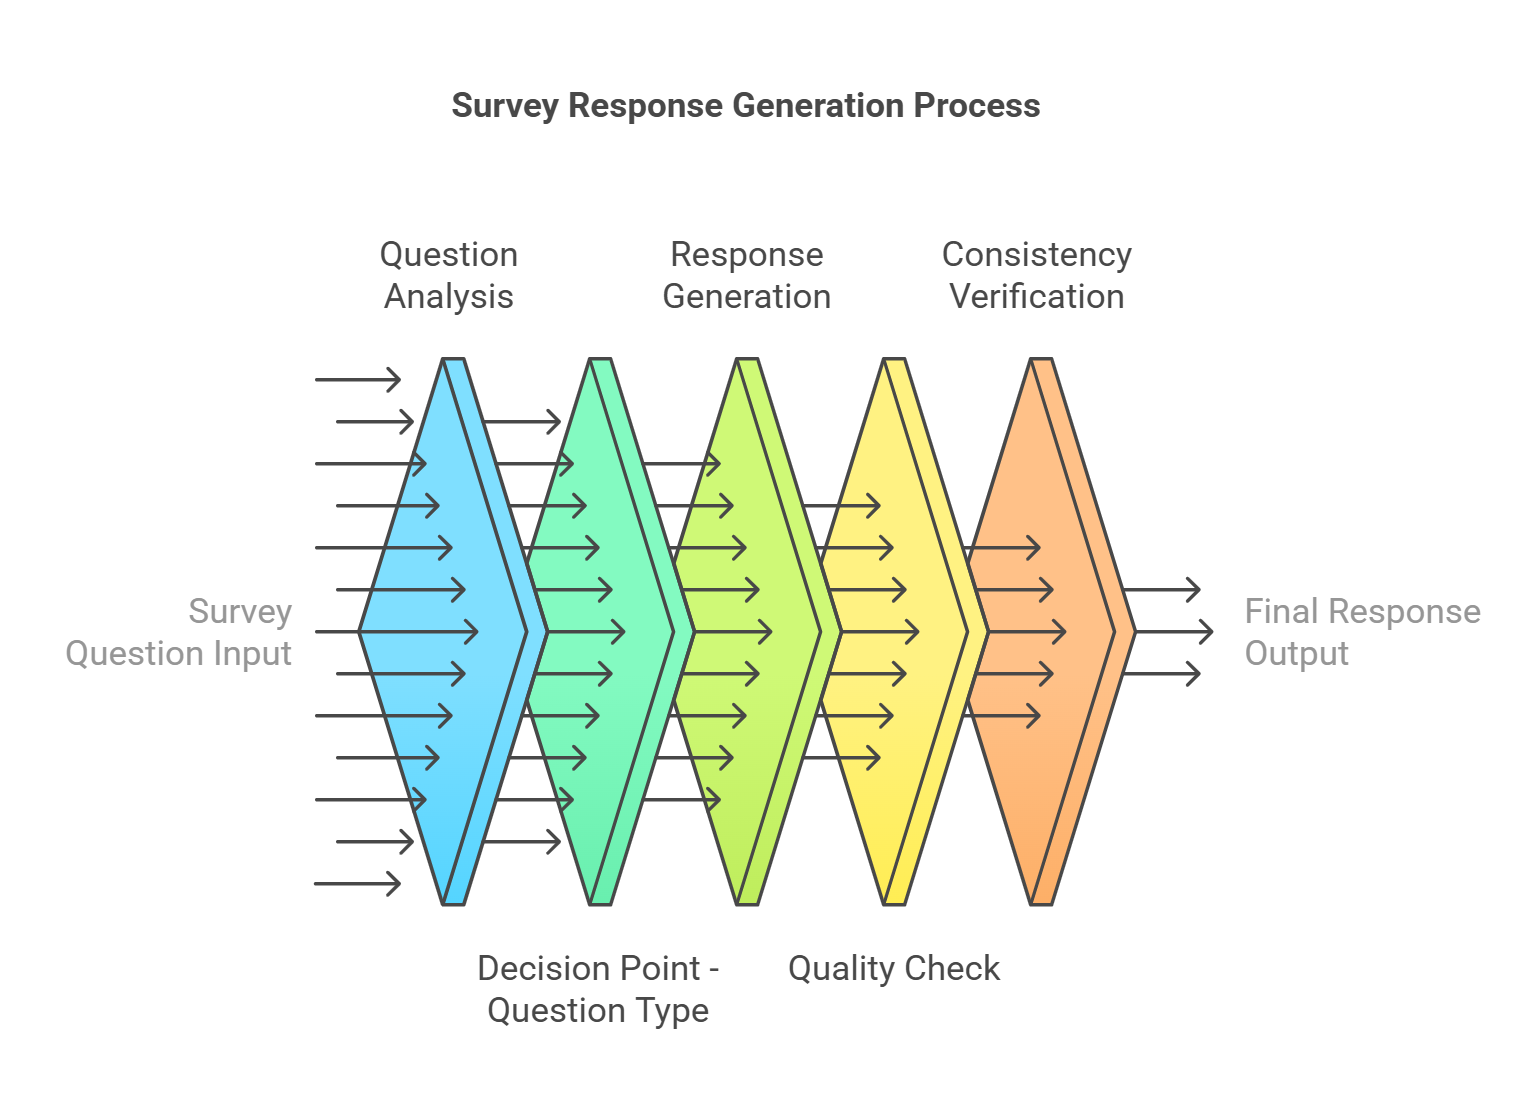
\includegraphics[width=1\linewidth]{latex//assets/PersonaVerse Response Generation Pipeline.png}
    \caption{A high level illustration of the process of survey response generation facilitated by persona-based Large Language Models}
    
\end{figure}

Current approaches in this area include the collection of survey response and analyis through simple rule-based response generation, statistical modeling of existing data, and recently, leveraging large language models to generate responses in the absence of any persona grounding. These approaches often lack the diversity of authentic human responses which possess consistency in demographic, behavioral, and psychographic characteristics across multiple questions.

We introduce the PersonaVerse framework, which facilitates the creation of persona-based agents capable of generating survey responses reflecting consistency in demographic and psychographic characteristics by leveraging large language models. When we approach grounding well-defined personas in response generation, it aims to create realistic and diverse synthetic responses compared to previous methods.

Our research offers several contributions, mainly: (1) method for instantiating LLM-Based agents for generation of responses to different question modalities possessing consistent persona characteristics; (2) a multifaceted framework for evaluating responses by assessment of quality, diversity and faithfulness in persona; and (3) an open source implementation for researchers to adapt according to various survey contexts. Although PersonaVerse does not replace human responses, it offers a complementary tool with the potential to improve. survey methodologies for research and reduce the barriers to the conduct of large-scale, diversified survey studies. Throughout our research, our aim has been to answer the following formulated research questions, to answer, which we believe are crucial for the outcome of our study:

\textbf{RQ 1}: To what extent can LLM agents maintain consistency in persona characteristics while generating survey responses across a variety of question modalities and topics?

\textbf{RQ 2}: How effectively can a swarm of persona-based LLM agents generate survey responses as compared to human respondents in terms of diversity and representative distribution?

\textbf{RQ 3}: What practical applications and limitations pose in the synthetic responses generated by persona-infused LLM agents within research and commercial context? 

\section{Related Work}
\begin{figure*}[t]
  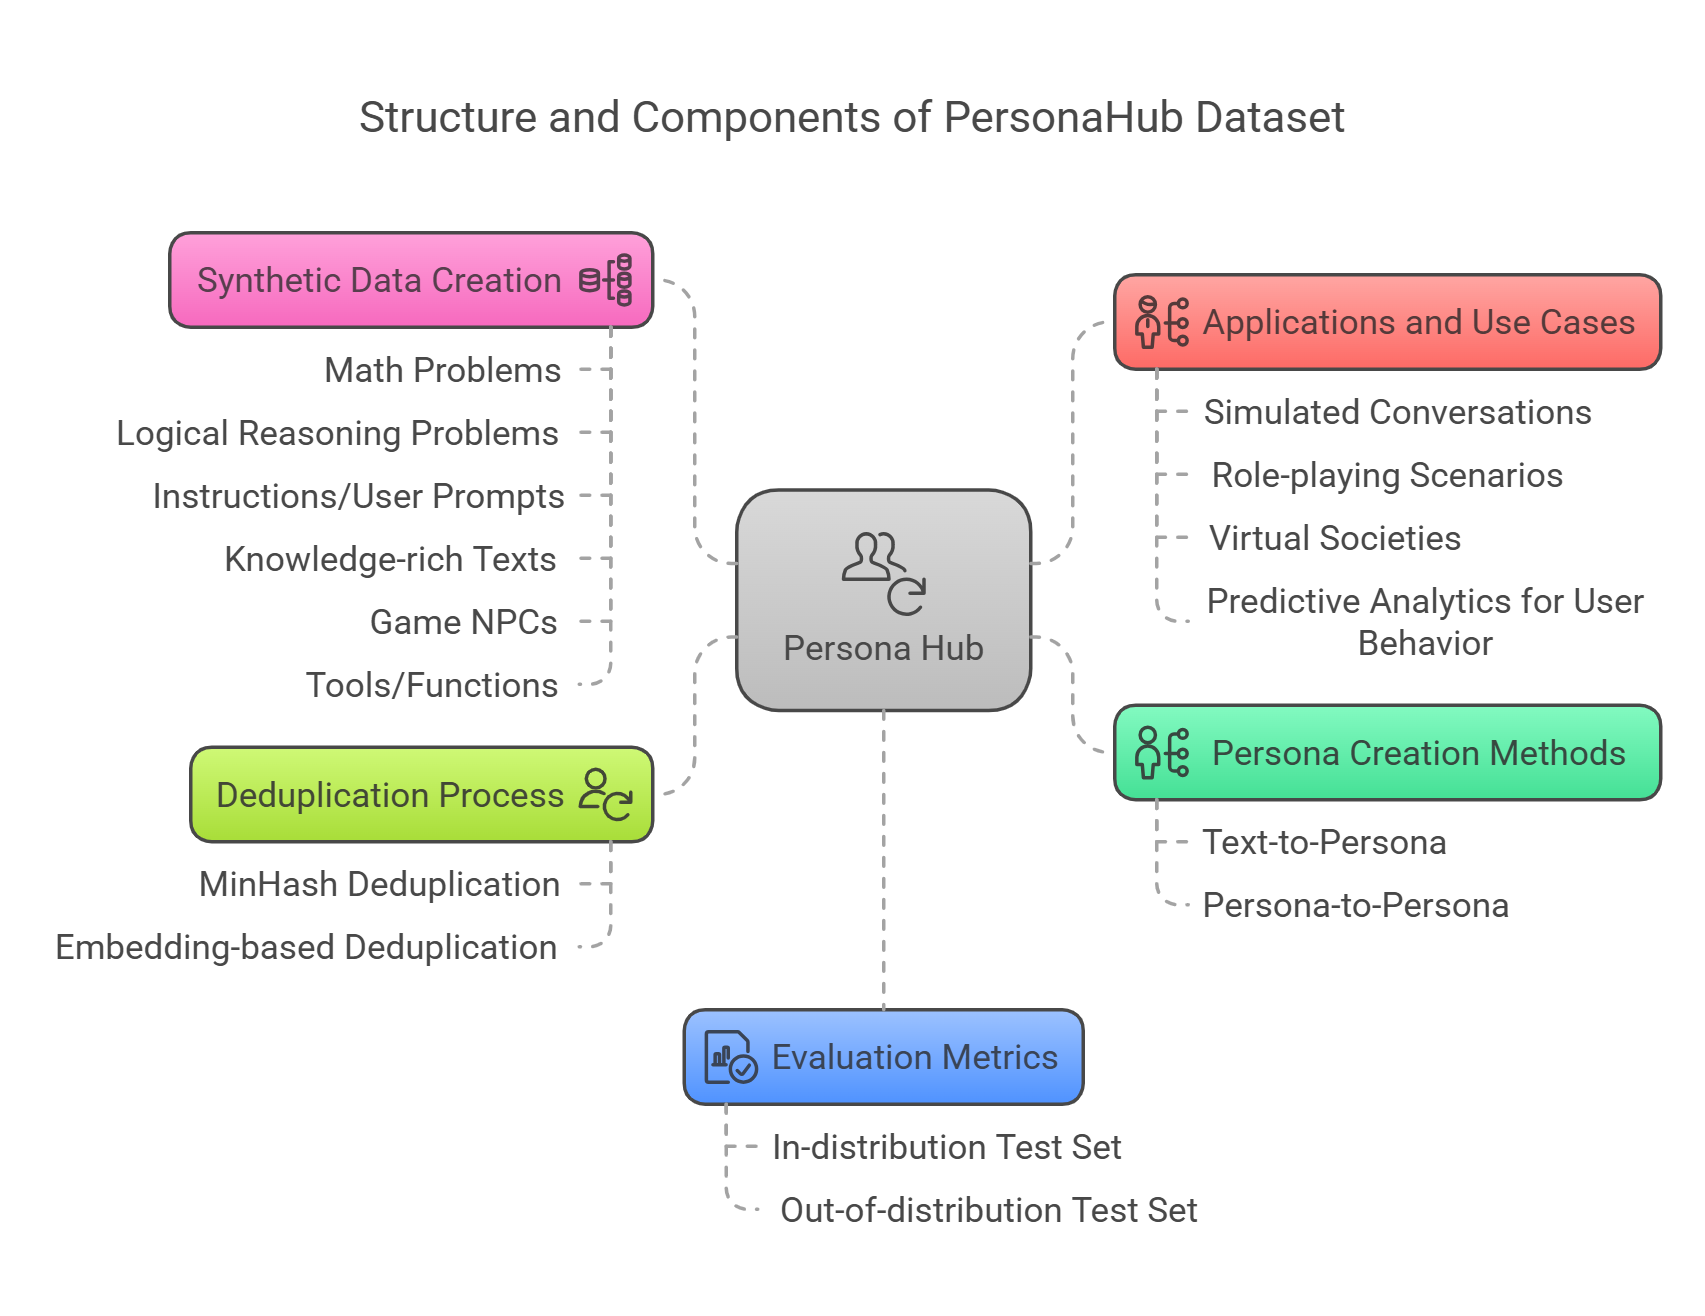
\includegraphics[width=0.48\linewidth]{latex/assets/Structure and Components of PersonaHub Dataset.png} \hfill
  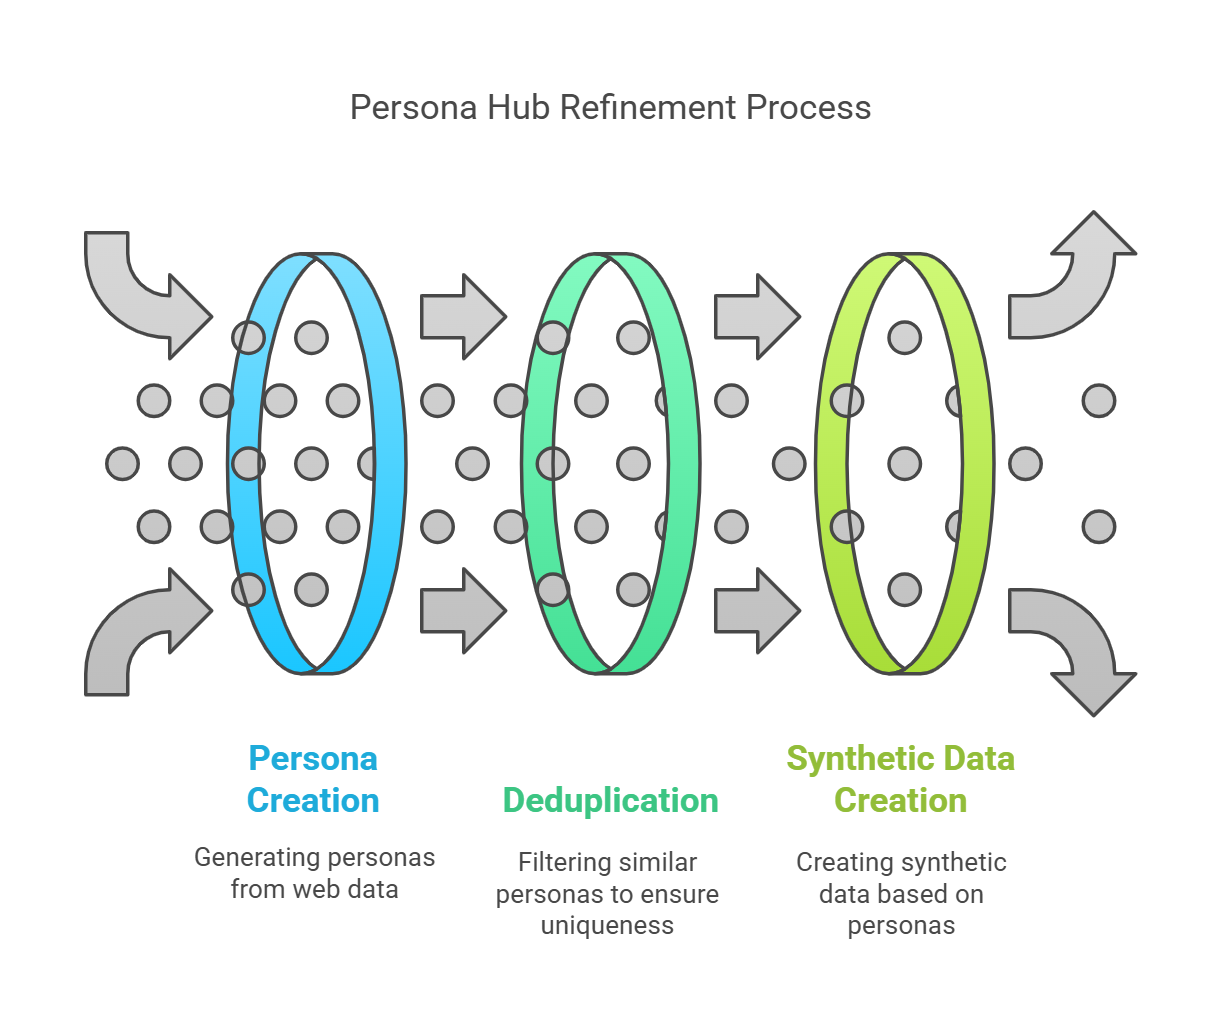
\includegraphics[width=0.48\linewidth]{latex/assets/PersonaHub Refinement Process.png}
  \caption {PersonaHub Dataset Structure, Components and Refinement Process}
\end{figure*}
Synthetic Data Generation in itself has not been a relatively new topic or domain of research. Multiple studies have proposed a variety of methods for the creation of synthetic data. In this section, we shall be going through selected literature that explores this area closely and resonates with our topic of research.

\subsection{Synthetic Data Generation}

With the growing need to address challenges related to data scarcity, privacy concerns and need for diverse domain based robust AI training, synthetic data generation has proven to be a pivotal solution. There have been numerous innovations, early on, with survey methodologies such as Address-based Sampling (ABS), and mixed-mode data collection which claim to have improved representativeness with minimal bias but gaps still exist in fully addressing the issue of selection bias \citep{annurev:/content/journals/10.1146/annurev-soc-060116-053613}.  Machine Learning applications have also leveraged generative models like GANs for synthetic data generation for the applications of classification tasks in the domain of healthcare and finance. While generative models perform this job effectively, challenges exist in capturing the complexity possessed by the real world \citep{9677302}. Advances in the field of generative AI, especially with the advent of Large Language Models like GPT-3, the capability of enabling domain-specific synthetic data generation has become possible using techniques like prompt engineering and parameter efficient tuning (PEFT), to name a few. But the biggest concern is that of hallucination and ethical considerations \citep{guo2024generativeaisyntheticdata}. Making use of S-BERT-based synthetic data generation pipelines, semantic similarity between survey items has been shown to influence response patterns with results showing successful replication of human factors, but the limitation of handling negations as well as scaling across diverse survey types and modalities still prevails \citep{10906589}

\subsection{LLMs for Text generation}

With the rise of LLMs and their role in advancing Natural Language Processing tasks which includes synthetic data generation, a tool such as DataDreamer \citep{patel-etal-2024-datadreamer} provides a unified framework to address challenges of scalability and reproducibility in LLM-driven synthetic data generation, fine-tuning, and other similar research workflows. SynthIE \citep{josifoski-etal-2023-exploiting} is another such innovative approach that exploits task asymmetry for the genration of high quality synthetic datasets. A similar framework, SynDG \citep{bao-etal-2023-synthetic} generates synthetic grounded dialogues which are modeled through dialogue flows and filter strategies applied to enhance coherence and quality of the system. In the domain of text classification, the potential of LLMs has depicted that low-subjectivity tasks benefit more from synthetic data generation methods \citep{li-etal-2023-synthetic}.  Authors of CodecLM use instruction tuning to tailor synthetic data for specific tasks using metadata encoding and refining the output iteratively, leading to superior results with diverse instructions. Finally, \citep{long-etal-2024-llms} provide a comprehensive survey emphasizing the need for unified methodologies in the curation, generation and evaluation of such synthetic data for multiple NLP workflows. Some of the common gaps identified, include biases in LLM outputs, issues of coherence in dialogue and challenges in adapting to domain specific applications 

\subsection{Persona-Based Generation}

The importance of modeling human-like behaviors and belief were explored soon after the prior research successfully made advancement in persona-driven survey response generation. A Generator-Critic architecture was introduced \citep{jandaghi-etal-2024-faithful}, which efficiently facilitated creation of high-quality persona datasets addreessing limitations in prior datasets such as Persona-Chat \citep{zhang-etal-2018-personalizing}. Although their approach demonstrated improvement in persona diversity, yet it struggled with intangible human traits like humor. In \citep{joshi2024personaswaymodeltruthfulness}, the authors cluster agents into personas which enhances truthfulness in noisy datasets, although challenges remained in defining the latent features that captured truthful personas reliably. Similarly, \citep{giorgi-etal-2024-modeling} evaluate explicit and implicit personas in order to replicate human biases. While explicit personas gave mixed results in takss such as belief geenration, implicit personas completely failed to align with human level of subjectivity. The inability ot consistently replicate biases in human responses across surveys designs was highlighted \citep{tjuatja2024llmsexhibithumanlikeresponse}, with RLHF-trained models introducing unwanted sensitivity despite marginal improvements in replicating human-like behavior. Finally, belief networks was proposed \citep{chuang2024demographicsaligningroleplayingllmbased} for the survey data to be enhanced in alignment with human opinions beyond role-playing on a demographic level. Although performance improved in temrs of reduced errors, yet broader applicability failed to achieve die to its simplistic structure with limited scope.

\begin{table*}[ht]
    \centering
    \begin{tabular}{|p{4cm}|p{6cm}|p{6cm}|} \hline  
         \textbf{Method} & \textbf{Benefits} & \textbf{Gaps} \\ \hline  
         
         Traditional Synthetic Data Generation & 
         - Addresses data scarcity and privacy concerns effectively. \newline
         - Enables domain-specific data creation using techniques like prompt engineering and PEFT. \newline
         - S-BERT pipelines replicate human factors in surveys. & 
         - Struggles with selection bias and accurately capturing real-world complexity. \newline
         - Hallucination and ethical concerns remain significant challenges. \newline
         - Limited ability to handle negations and scale across diverse survey types and modalities. \\ \hline  
         
         LLMs for Text Generation & 
         - Tools like DataDreamer and SynthIE enhance scalability, reproducibility, and coherence. \newline
         - Instruction tuning (e.g., CodecLM) improves task-specific synthetic data generation. \newline
         - Unified frameworks improve curation, generation, and evaluation of synthetic data. & 
         - Biases in outputs, coherence issues in dialogues, and domain adaptation challenges persist. \newline
         - Low subjectivity tasks benefit more, limiting broader applicability. \newline
         - Ethical concerns and lack of consistency in domain-specific applications remain barriers. \\ \hline  
         
         Persona-Based Generation & 
         - Generator-Critic architecture improves persona dataset quality and diversity. \newline
         - Enhances truthfulness in noisy datasets through persona clustering. \newline
         - Belief networks align survey data with human opinions beyond role-playing demographics. & 
         - Struggles with intangible traits like humor and human subjectivity. \newline
         - Challenges in defining latent features for reliable truthful personas persist. \newline
         - Simplistic structure limits broader applicability across diverse scenarios. \\ \hline  
    \end{tabular}
    \caption{Qualitative comparison of methods discussed in Section 2.}
    \label{tab:comparison}
\end{table*}

\section{Dataset}

At the time of drafting this research project proposal, we find the PersonaHub Dataset provided by Tencent AI Lab \citep{ge2024scalingsyntheticdatacreation} highly promising. In this section we shall discuss more about the dataset and how can it help us achieve our use case. This dataset introduces a person-driven approach for creation of synthetic data at scale making use of 1 billion personas curated from web data. Although the complete dataset has more than 1 billion personas, we shall be exploring only the tiny subset of 200,000 personas furthermore narrowing down to a couple of 1000s keeping in mind the computational resources we possess. As per the authors, these personas act as distributed carriers of the world's information, enabling LLMs synthesize this dataset across various domains including math, logical reasoning, game NPC persona development, instructions, tools and knowledge-rich texts.
For our research we plan to utilize the detailed persona descriptions that include demographic information, personality traits, interests, values, behavioral patterns, etc derived from this dataset. A structured format for these personas shall be created such that enables their use in effective conditioning of language model outputs. Rather than using the PersonaHub dataset out-of-the-box, we plan to develop a methodology for creating persona descriptions by giving them structure and then use it to adapt to different contexts and requirements.
The Figure 2. shows the various components of the PersonaHub Dataset.
We also plan to compile a diverse collection of survey questions spanning multiple domains such as:
\begin{itemize}
    \item Consumer behavior
    \item Consumer preferences
    \item Social, Political attitudes
    \item Technology adoption and usage
    \item Healthcare
\end{itemize}
As per the modalities of the survey questions, we aim to cover the following four most frequently used modalities, providing the capability to geenrate responses for:
\begin{itemize}
    \item Multiple Choice-type questions
    \item Likert scale based
    \item Ranking based
    \item Open-ended questions
\end{itemize}
For evaluation purposes, we aim to make use of two types of datasets: (1) Human benchmark responses, which are publicly accessible survey data from established sources; (2) Expert evaluations, which shall be used to assess response quality and consistency in persona.
\begin{table*}[ht]
  \centering
  \begin{tabular}{|p{3cm}|p{5cm}|p{3cm}|p{5cm}|}
    \hline
    \textbf{Base Language Model} & \textbf{Reason} & \textbf{Embedding Models} & \textbf{Reason} \\
    \hline
    LLaMA-2-7B & Default choice for response generation & Sentence Transformers & Default choice for embeddings \\
    \hline
    Mistral-7B & Consistent output quality; variants optimized for question answering and instruction following & Universal Sentence Encoder (USE) & Fast inference, fine-tuned for question-answering tasks \\
    \hline
    FLAN-T5 & Excels in multi-task learning & DistilBERT & Faster inference; minimal performance trade-offs \\
    \hline
    Gemma2 & Lightweight; efficient; suitable for real-time applications & fastText & Ideal for simple tasks; efficient text classification \\
    \hline
  \end{tabular}
  \caption{Proposed Base Language Models and Embedding Models}
\end{table*}
\begin{table*}[ht]
  \centering
  \begin{tabular}{|p{3cm}|p{5cm}|p{3cm}|}
    \hline
    \textbf{Metric}& \textbf{Focus Area}& \textbf{Tools/Methods}\\
    \hline
    Faithfulness& Response Quality& Semantic Alignment Tools\\
    \hline
    Relevance& Response Quality& AI Assisted Scoring (1-5 Scale)\\
    \hline
    Coherence& Linguistic Quality& Perplexity, Human review\\
    \hline
    Similarity& Reference Alignment& BLEU, ROGUE\\
    \hline
 Persona Consistency& Persona Alignment&Thematic Analysis\\\hline
  \end{tabular}
  \caption{Summary Table for Proposed Evaluation Metrics}
\end{table*}
\section{Methodology}

On a high level, we divide our proposed research project implementation into two modules: 
\begin{enumerate}
    \item Persona Agent Creation \& Management Module
    \item Survey Management \& Question Processing Module
\end{enumerate}
\subsection{Persona Agent Creation \& Management}
The Persona Agent Creation and Management module establishes and keeps different persona agents which use large language models (LLMs). System initialization requires executing the loading of pre-trained LLMs and embedding models during which performance optimization techniques particularly 4-bit quantization are applied. The Personas can be imported from structured data sources that include DataFrames to generate semantic embeddings with advanced sentence embedding models. The embedding technology groups personas into similar clusters based on semantic relationships which improves the success of organization and retrieval operations. Through its design the system enables detailed persona description storage which links to distinct identifiers for creating agent profiles. The agents produce detailed authentic survey responses by utilizing specialized prompt templates alongside LLM pipelines. The system permits users to generate batch responses and export results to CSV or JSON structure then store outputs for analysis. The system structure enables the management of various research-specific agents through adaptability features combined with scalability measures.

\subsection{Survey Management \& Question Processing}
This module serves as a complete system to build and handle surveys. Through the system users can build surveys that include exclusive identifiers and titles with descriptions alongside the capability to draw survey questions from various predefined templates. A combination of multiple-choice questions and Likert scale questions as well as open-ended questions and yes/no questions and ranking questions are supported by the platform. The module facilitates the addition of questions to a centralized question bank and their subsequent association with specific surveys. Dynamic question generation lets users specify their areas of interest which activates templates and randomization for creating diverse relevant inquiries. The system allows users to customize their surveys through options that help set Likert question scales and create specific ranking and multiple-choice question answer sets for better adaptability. The system allows users to import and export surveys through JSON format which facilitates smooth data exchange between different projects. The system's features combine to simplify survey development while handling various research situations effectively.
\begin{figure}[t]
  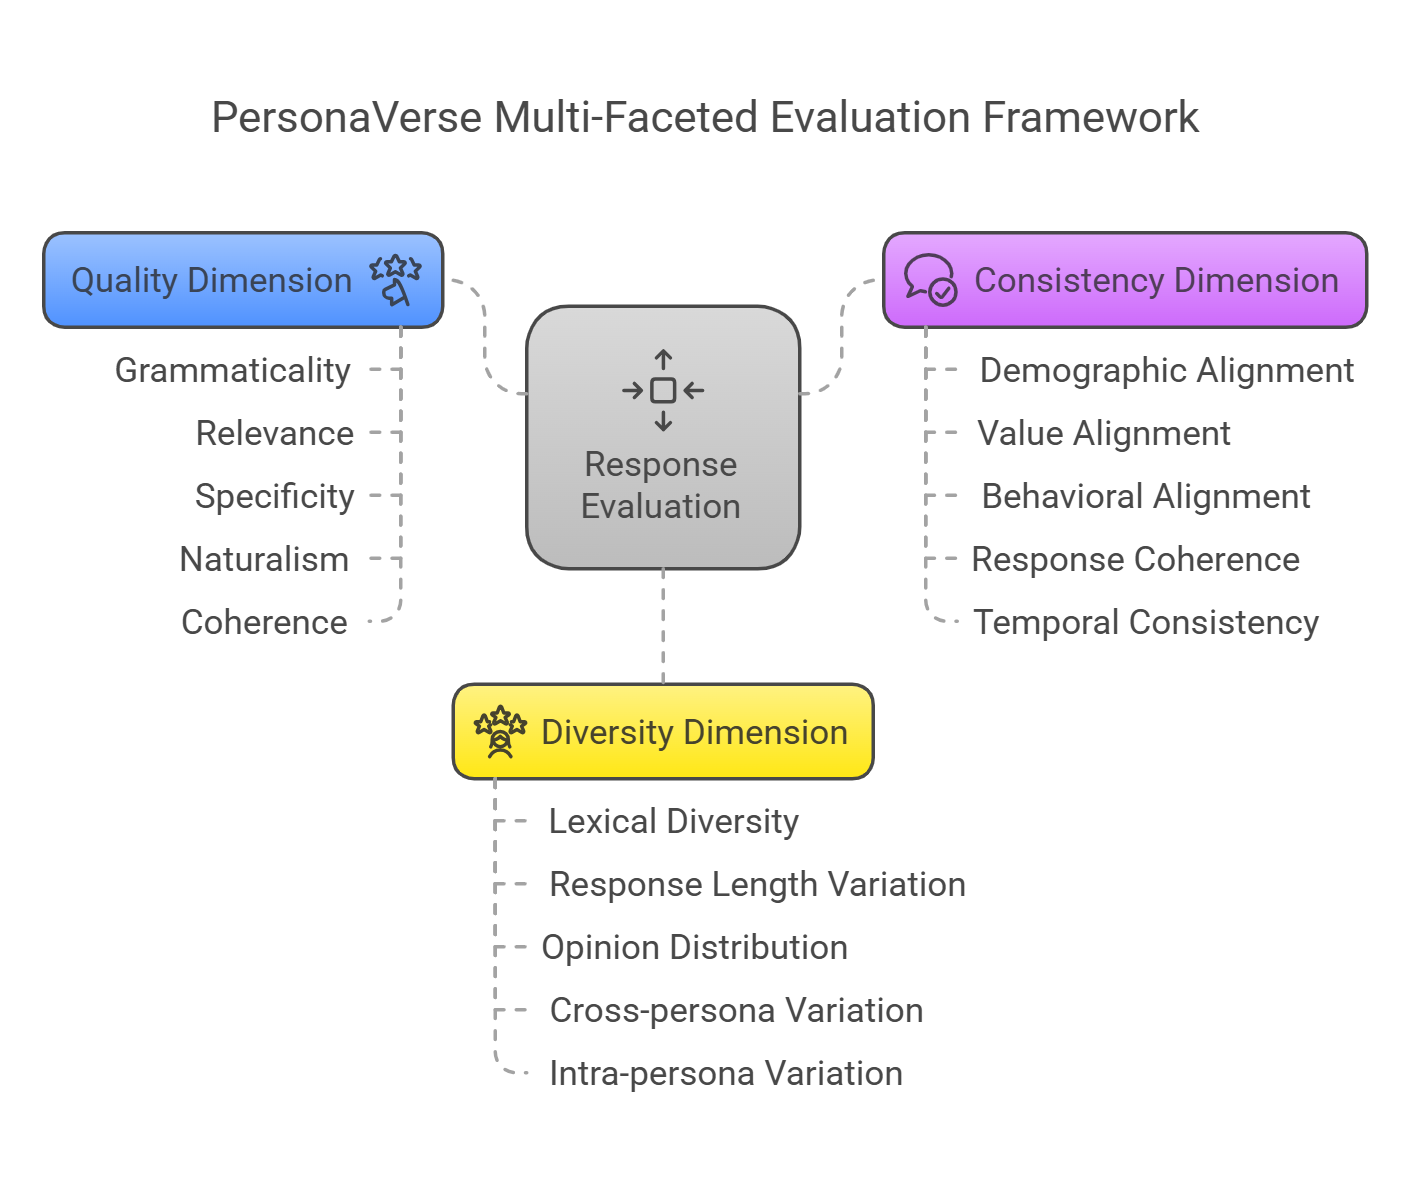
\includegraphics[width=\columnwidth]{latex//assets/PersonaVerse Multi-Faceted Evaluation Framework.png}
  \caption{A high level multi-faceted evaluation framework covering the three dimensions of evaluation namely: Quality, Consistency and Diversity with respect to persona-based synthetic response generation}
\end{figure}

\subsection{Response Generation Pipeline}

Our proposed pipeline for response generation operates to generate survey answers which maintain high quality content along with relevant context through reliable output mechanisms.
The system uses dynamic approaches to create responses per survey question classification. The system creates responses using provided templates together with question-related context to generate answers which match the specified question format (such as Likert scales or multiple-choice or open-end). The generative models generate cohesive detailed answers for open-ended questions and select or compose responses for structured formats such as ranking and yes/no questions to match predefined criteria. The response-generation strategies produce answers that meet both the requirements for survey variety and accurate correspondence to the intended survey design.
Data reliability depends on the pipeline's requirement for standardized responses through system-implemented logical frameworks and scaled uniformity. These logical verification systems enable different survey answers to stay compatible with one another and maintain a flowing relationship between survey questions. The survey logic enables consistently linked answers when a respondent shows satisfaction within a particular question. 

\subsection{Training}

The way we envision the creation of the PersonaVerse Framework, our current approach relies on the Agentic AI paradigm currently limited to the use of existing language models.  We provide a table of models we wish to compare and make use of in this project, as mentioned in Table 2.
The rationale behind doing so is to focus on effective prompting and context management with pre-trained models thereby reducing computational requirements, ease of accessibility to researchers with limited resources, and the flexibility to incorporate new and improved models as and when they are released and made available to the general public.
Yet, as part of our experiments we aim to instruction tune a base language model specific to our use case and make use of that model as our base model. The PersonaHub Dataset shall be utilized in generating instruction data for the mdoel to train on and we shall resort to intemrediate methods like distillation i.e, generating rich data from large, proprietary models and then tune our models using the generated data. 
As per computational availability and count of resources, we shall be making use of institute's Puffer serversd along with a Google Colab Pro Subscription providing us access to NVIDIA T4, P100, L4, and potentially A100 GPUs. Our trained/fine-tuned models shall be pushed to Hugging Face Hub for quick inference via its API.

\subsection{Evaluation / Metrics}

The evaluation process of the Persona-Based Survey Response Generation system requires measurement of AI response quality in addition to system operational effectiveness. The evaluation of created responses requires metrics that measure three things: faithfulness, relevance, coherence as well as similarity. The evaluation of persona descriptions adherence depends on faithfulness measurement through semantic alignment tools. The relevance evaluation determines how well AI-generated survey answers correspond to the original questions while also allowing 1-5 scoring assessment through AI tools. Coherence stands as an evaluation aspect that determines both logical structure and linguistic fluency and it can be assessed through perplexity analysis or human assessments while similarity measurements utilize BLEU and ROUGE when comparing generated responses to reference texts. Table 3. summarizes the proposed evaluation metrics as part of the project.
Persona alignment plays a vital role in evaluation because it checks that responses maintain congruity with the specified persona traits. Commentary on persona consistency functions as an evaluation metric because thematic analysis reveals repeatable themes that confirm how well the responses match persona attributes. Adding these evaluation metrics to the project allows complete assessment of both system technical achievement and practical functionality to validate effective objective fulfillment.

\section{Discussion}

The PersonaVerse framework serves survey research methodology by delivering researchers the capability to create natural yet authentic survey answers representing multiple human viewpoints. The framework shows proof of its usefulness for key research questions through its unification of persona descriptions with advanced language models in addition to evaluation methods. The structural application of detailed persona attributes in agent prompts results in response consistency that tracks persona characteristics through evaluation frameworks to measure alignment in RQ1. Empirically, it has been proven that suitable prompt engineering enables language models to maintain high consistency for explicit persona characteristics but presents difficulties when reasoning implicitly. RQ2 utilizes diversified persona descriptions among demographics and psychographics to enable cluster-based respondent pooling suitable for research requirements. The combination of approaches has yielded a greater level of response diversity and supports experimental evaluations into response-influencing variables according to preliminary analysis. With regard to Practical Utility as mentioned in RQ3 the system integrates seamlessly with survey platforms and includes demographic distribution specification tools alongside features for generating multiple survey response types. The method demonstrates worth when researchers use it prior to conducting surveys to test questionnaires and develop theoretical distributions of responses by population subsets thus helping research design and statistical power evaluation. Such advances in software often overshadow the existing drawbacks such as model biases together with data dependence and the unattainable goal of human data elimination. The research team implements ethical protocols that include detecting bias automatically and providing detailed documentation about limitations together with established rules that indicate proper use scenarios to make PersonaVerse work as an additional tool instead of replacing traditional survey methodologies.

\section*{Summary of Progress}

As of the day of submission of this proposal report, here is the summary oif the progress we have made so far:
\begin{itemize}
    \item Reviewed around 20 papers, understanding the core implementations, available methods and existing approaches
    \item Setup the \href{https://github.com/users/aryashah2k/projects/2}{Kanban Board} on Github \citep{Shah_All_the_world_s_2025} for effective Project Management and Planning
    \item Procured the dataset and beginning heuristic exploration of the dataset and its utility in creation of agents for our tasks
    \item Set up CI/CD Pipelines for our project, utilizing \href{https://github.com/aryashah2k/PersonaVerse/tree/main/.github/workflows}{GitHub Actions}
\end{itemize}

\section*{Acknowledgments}

The authors thank Dr. Chaklam Silpasuwanchai of Asian Institute of Technology, Thailand, for providing the guide on Wobbrocks 5 part structure, helping in brainstorming topic ideas and motivating us for the research topic presented in this paper

The authors also thank Mr. Todsavad Tangtortan for providing insights and checking our work throughout our experimental study and research phases, along with introducing us to various best practices and sample code snippets that the current project derives inspiration from.

% Bibliography entries for the entire Anthology, followed by custom entries
%\bibliography{anthology,custom}
% Custom bibliography entries only
%\bibliography{custom}
\bibliography{latex/custom}

%\appendix

%\section{Appendix}
%\label{sec:appendix}

%This is an appendix, it shall be filled as we progress through this research project.

\end{document}
